\section{Applications}
\label{clicknp:sec:application}

The following will discuss these network functions in detail.

%
\egg{
To handle the large traffic volume in datacenters, it requires the L4LB to support up to 32 million flows in the flow table.
Clearly, such a large flow table cannot fit into the BRAM of FPGA, and has to be stored in onboard DDR memory.
Accessing DDR memory is slow. To improve performance, we further create a 4-way associative flow cache in BRAM with 16K 
cache lines. The flow cache is replaced based on the Least Recently Used (LRU) algorithm.
DDR memory access is a fat pipeline stage as shown in Figure \ref{clicknp:fig:unbalance}. We move the DDR access part to a separate element to make the fast path run asynchronously with slow path.}

\egg{
pFabric \cite{alizadeh2013pfabric} is a near-optimal datacenter transport based on priority scheduling and dropping. Packets are scheduled based on its flow size or remaining flow size in a small queue. Our pFabric scheduler implementation (Figure \ref{clicknp:fig:PFabric}) support 4-giga strict priorities, including a PriorityQueue which deques the packet with highest priority and drops overflow packets with lowest priority, a ReorderQueue to find the earliest packet from the flow with highest priority to avoid starvation and keep packet ordering, and a PacketBuffer to receive packets into buffer and schedule or drop packets out of buffer. Since queue size in a perfectly load balanced fabric should be small, we choose shift register priority queue for maximum throughput and clock frequency.

ReorderQueue is another shift register queue ordered by flow hash. On enque command from PacketBuffer, packet metadata with flow hash $f_{new}$ is enqued to entry $i$ where $f_{i-1} < f_{new} \leq f_{i}$. On deque command from PriorityQueue, the entry $i$ with $f_{i} = f_{deque} < f_{i+1}$ is dequed. Packets with a same flow hash are dequed in the same order as they are enqued.

\begin{figure}[h!]
	\centering
	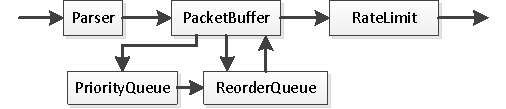
\includegraphics[width=1.0\columnwidth]{image/PFabric}
	\vspace{-0.30in}
	\caption{PFabric Element Graph}
	\vspace{-0.10in}
	\label{clicknp:fig:PFabric}
	%    
\end{figure}
}

